\chapter{Auswertung / Experiment / Vergleich mit Property-based Testing}

\section{Vergleichmetriken}
Bevor wir einen tatsächlichen Vergleich beider Methoden durchführen werden erst einmal die Metriken eingeführt in denen
sich Verglichen wird.
Hierdurch wird einfacher verständlich welche Punkte miteinander verglichen werden.
Wir werden einige neue Metriken einführen aber auch Metriken nutzen die in \textit{Property-based Testing}\cite{property-based-testing} genutzt wurden.

\subsection{Metriken aus Property-based Testing}

In \textit{Property-based Testing} wurden zwei Metriken eingeführt, um die Methode zu evaluieren.
Hierbei wurden zwei Forschungsfragen entwickelt.

\begin{enumerate}
    \item Welche Schema Coverage kann mit der Methode erreicht werden? \cite[vgl. RQ1]{property-based-testing}
    \item Wie gut ist die Fehlerfindungskapazität der Methode? \cite[vgl. RG2]{property-based-testing}
\end{enumerate}
\caption{Forschungsfragen aus Property-based Testing}

Zur Auswertung der Methode wurden zwei Testsysteme genutzt.
Das erste Testsystem ist eine eigens entwickelte GraphQL-API die bekannte Fehler besitzt \cite[vgl. A.1]{property-based-testing}.
Testsystem 2 ist GitLab.
Ein häufig genutztes Tool für GitServer mit DevOps Kapazitäten.
Gitlab bietet seine API auch als GraphQL an und durch seine riesige Größe eignet sich GitLab als solides Testsystem. \cite[vgl. A2]{property-based-testing}
Unser entwickelter Prototyp soll in exakt dem gleichen Umfeld seine Tests generieren.
Wir erwarten, dass wir möglichst die selben Fehler finden wie die ursprüngliche Methode und positiv wäre, wenn wir mehr und neue Fehler finden würden.
Beide Forschungsfragen werden im folgenden nocheinmal näher erläutert da diese ein wenig spezialisiert sind und Wissen über Methode
ist wichtig um die Ergebnisse korrekt einordnen zu können.

\subsection{Fehlerfindungskapazitäten}

Mit Fehlerfindungskapazitäten ist gemeint wie zuverlässig die Methode tatsächliche Fehler findet.
Hierfür werden die beiden zuvor benannten APIs getestet und es wird geprüft ob die Methode die Fehler finden konnte.
Um zu verifizieren, dass die Methode möglichst viele Fehler findet gibt es eine Test API die
initial mit bekannten Fehlern versehen wird.
Die \textit{Property-based Methode} hat 11 von 15 Fehlern im speziell vorbereiteten System gefunden.
Bei GitLab wurden 15 bugs gefunden.
Unsere entwickelte Methode soll mindestens die gleichen Fehler finden und idealerweise mehr.

\subsubsection{Schema Coverage / Schema (Ab)Überdeckung}

Dadurch, dass \textit{Property-based Testing} auf zufallsbasierter Testgenerierung basiert stellt sich hier die Frage, wie gut die Methode
die API abdeckt und inwiefern die generierten Tests ausreichend sind.
Dies kommt insbesondere zu tragen, wenn die maximale Pfadlänge ausgehend vom Query Knoten größer ist als die erlaubte Rekursionstiefe des Prototypens.
In Property-based Testing wird definiert, dass die generierten Tests eine Full-Schema Coverage erreichen, wenn gilt:

\begin{definition}
    Für alle Objekte des Schemas: Bilde alle Tupel \{Object, Field \}.
    Ein Schema hat eine ideale Coverage wenn alle Tupel durch einen Test abgedeckt sind.
\end{definition}

Wie in Property-based Testing schon erwähnt: \textit{da keine Coverage Metric für GraphQL Blackbox Test Auswertung exisitiert, starten wir mit einem sehr
einfachen und intuitiven Ansatz}~\cite[vgl. B. Measuring Schema Coverage]{property-based-testing}.
In der Tat ist das vorgestellte Coveragekriterirum ein sehr einfaches Kriterium.
Es lässt zum Beispiel die Beziehungen zwischen allen Knoten aus und beachtet nur, dass alle Knoten inbegriffen sind mit allen Feldern.
Hiermit entspricht das definierte Coverage-Kriterium einer Kombination aus Edge- und Nodecoverage.
Denn alle Knoten müssen abgedeckt sein und alle Kanten ausgehend von den Knoten.
Wie zuvor gesehen ist ein solches Kriterium allerdings noch nicht ausreichend für eine ideale Testabdeckung, da
zum Beispiel die verschiedenen Kantenkombinationen außer acht gelassen werden und sich somit doch noch Fehler im Code befinden können.
Wesentlicher Unterschied beider Methoden ist insbesondere, dass \textit{Property-based Testing} überprüfen muss ob es diese Coverage erreicht.
Unsere vorgestellte Methode stellt sicher, dass diese Coverage erreicht ist bevor sie aufhört mit dem generieren.
Die Überprüfung der Schema-Coverage in Property-based Testing geschah durch ausprobieren.
Hierbei wurde ausprobiert wie viele Testgenerierungen benötigt wurden, um das definierte Kriterium zu erfüllen.
Um ein 100\% Coverage beim GitLab Schema zu erreichen waren verschiedene Anzahlen an Iterationen nötig bei verschiedenen Rekursionslimits.
Eine 100\% Coverage wurde bei GitLab nur erreicht wenn 10000 Tests mit Rekursionslimit 4 erstellt wurden.
Die Berechnungszeit war hierbei 931 Sekunden.
Dies ist zwar der schlechteste Wert in der gesamten Statistik und man könnte meinen, dass der Vergleich
nun nicht genau wäre - allerdings ist dies auch der einzige Wert der verlässlich 100\% Coverage geliefert hat.
Unser Ziel ist es also, weniger als 10.000 Tests und 930 Sekunden zu benötigen um das hier definierte CoverageKriterium zu erfüllen.

\subsection{Neue Metrik}

Näheres betrachten des Codes von \textit{Property-based Testing} offenbarte einen signifikanten Fehler in der Definition der Schema Coverage.
Hierbei ist besonders wichtig zu wissen, wie GraphQL unter der Haube funktioniert.
GraphQL verarbeitet die Schritte einer Query sequentiell.
Nutzen wir die zufällig generierte Query aus \textit{Property based Testing Fig. 9}\cite{property-based-testing}.
Die Query lautet:
\begin{lstlisting}[language=GraphQL]
    {projects(id: "7x8Z"){description members{name}}}
\end{lstlisting}

Stellen wir nun diese Anfrage an die API und es existiert kein $Project$ mit der id 7x8Z so hat die Funktion
einen return Value von $null$.
Ein Return Value von null bedeutet jedoch, dass GraphQL den Pfad nicht weiter auswerten wird und die Funktion des Resolvers hinter dem $members$ Feld nicht ausgeführt wird.
Diese Query würde jedoch die Coverage für die Tupel Project und Members erfüllen aus der vorigen Definition, ohne, dass diese wirklich getestet wurde.
Laut Property-based Testing wird hierdurch angenommen, dass die Query erfolgreich ist wenn die Query erfolgreich ist.
Allerdings haben wir nun ungetesteten Code der als getestet betrachtet wird.
Wir wollen nun eine Metrik einführen die überprüft wieviel der zufällig generierten Querys tatsächlich komplett getestet haben.
Hierfür wird folgende Metrik eingeführt:

\begin{definition}
    Für alle Querys und dazugehörigen Responses wird die Pfadlänge bestimmt.
    Eine erfolgreiche Query hat dann zwei mögliche Szenarien:
        \begin{enumerate}
            \item Pfadlänge(Query) = Pfadlänge(Response)
            \item Pfadlänge(Query) > Pfadlänge(Response)
        \end{enumerate}
\end{definition}

Tritt Fall 1 ein so hat die Query wirklich alle Funktionen getestet.
Tritt Fall 2 ein so hat die Query nicht alle Funktionen getestet.
Zählt man nun alle Querys zusammen kann man auswerten zu wieviel Prozent die gesamte erwartete Pfadlänge tatsächlich ausgeführt wurde indem die Pfadlänge(Response) hinzugezogen wird.

\section{Threats to Validity / Limitierungen}

Bevor wir mit dem eigentlichen Vergleich beginnen muss noch kurz eingeordnet werden inwiefern die Experimente zu betrachten
sind und unter welchen Vorraussetzungen der Vergleich geschieht.

\subsection{Argumentgeneratoren}

Wie in $8.1.3$ angesprochen ist es wichtig, dass GraphQL für jede Funktionen einen Wert ungleich $null$ bekommt, sodass der
Pfad weitergegangen werden kann und die Funktionen in diesem getestet werden.
Um Bedingungen zu begünstigen werden die Argumentgeneratoren für jedes Experiment angepasst, sodass es sehr viel wahrscheinlich ist, dass
die generierten Argumente auch zum SUT passen und die allgemeine Query-Qualität hierdurch besser wird.
Es hängt dann explizit davon ab wie sehr die Argumentgeneratoren angepasst werden denn ein einfaches anpassen hat sich \textit{Property-based Testing}\cite{property-based-testing}
auch erlaubt.
Hierbei sei zum Beispiel erwähnt, dass eine Type $ID$ in GraphQL als String wert definiert ist, häufig in Implementierung jedoch als Zahlenstring genutz wird.
Eine beispielhafte Anpassung wäre hier nun, dass wir den Generator für den Type $ID$ so anpassen, dass er nur Argumente für  $ID$ zurückliefert die ein Zahlenwert sind
in einem gewissen Bereich der durch das SUT abgebildet wird.


\section{Fehlerfindungskapazitäten}

Zuerst wollen wir die Fehlerfindungskapazitäten des Testtool auf die Probe stellen.
Hierfür nutzen wir die beiden, zuvor benannten, Testsyteme GraphQL-Toy (eine experimentelle GraphQL-Implementierung) und GitLab in der Version 12.6.3.
Ziel ist es mindestens die Fehler zu finden die vom \textit{Property-based Testtool}\cite{property-based-testing} gefunden wurden.
Idealerweise wollen wir jedoch sogar mehr Fehler finden.

\subsection{GraphQL-Toy}

Das Testssystem GraphQL-Toy hat ein sehr simples Schema in dem nur drei $OBJECT$ Typen exisitieren.
Diese sind $Query$, $Project$ und $User$. 
Das Schema hat folgende Struktur: \\
\begin{center}
    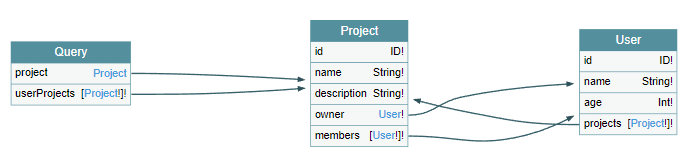
\includegraphics{img/graphqltoy}
\end{center}

Entwickelt wurde dieses System mit dem Hintergrund, dass bekannte Bugs im Code eingebracht werden und überprüft werden kann ob das Testtool diese findet.
Insgesamt wurden 15 verschiedene Buggs vorgestellt welche in verschiedene Kategorien fallen wie Syntaxfehler, falsche Rückgabedaten, falsche Datenstrukturen etc.
Einige der Bugs werden im folgenden kurz vorgestellt.
Eine Liste aller eingebauten Bugs lässt sich im Appendix unter \textit{GraphQL-Toy Implementation mit Bugs}~\ref{graphql-toy-code} finden.

\subsubsection{Bug 1 - SyntaxFehler}

Einfache Syntaxfehler wurden an verschiedenen Stellen eingebaut.
Dies bedeutet, dass jeder Funktionsaufruf dieser Funktion garantiert scheitern wird.
Somit kann jede Request diesen Fehlerfall entdecken, solange die Request auch das Feld hinter der Funktion mit dem Syntaxfehler abfragt.
Ein einfacher Syntaxfehler wäre zum Beispiel folgender Code: \\

\begin{lstlisting}[language=javascript]
    const resolvers = {
        Query: {
            project: (_, {id}, context, info) => {
                // Example bug 1 - Syntax mistake
                return db.projects.find(project => project.id ===);
            }
        }
    }
\end{lstlisting}

Hierbei fehlt der Wert mit dem die $project.id$ verglichen werden soll.
Ein jeder Aufruf dieser Funktion mit egal welcher $ID$ führt zu einem Fehler.

\subsubsection{Bug 2 - Falscher Objekttyp}

Objektfehler sind ein wenig unoffensichtlichere Fehler.
Hierbei gibt der Code ein Objekt zurück, dass nicht der definierten Struktur im Schema entspricht.
GraphQL wird hierfür dann einen Fehler erzeugen da die Daten eben nicht zum Schema passen.

\begin{lstlisting}[language=javascript]
    const resolvers = {
        Query: {
            project: (_, {id}, context, info) => {
                // Example bug 5 - wrong type "error"
                return { ...db.projects.find(project => project.id === id), name: ["a", "b"] };
            }
        }
    }
\end{lstlisting}

Um diesen Fehler ausführen zu können ist es wichtig, dass das Feld auch abgefragt wird.
Sollte das Feld ein Argument benötigen, so muss dieses passen, sodass auch wirklich ein Objekt abgefragt wird und dann der falsche Type zrückgegeben wird.

\subsubsection{Bug 3 - Typfehler in der Eingabe}

Felder wie $ID$ sind im GraphQL-Standard als einzigartige Strings definiert.
Im allgemeinen wird der $ID$ Type jedoch von diversen Entwicklern als Zahlenstring genutzt.
Eine Funktion wandelt diesen String dann in eine Zahl um die z.B. genutzt wird um einen bestimmten Eintrag eines Arrays zu bekommen.
Inputvalidierung ist also von Nöten.

\begin{lstlisting}[language=javascript]
    const resolvers = {
        Query: {
            project: (_, {id}, context, info) => {
                // Example bug 3 - Input type validation bug
                return db.projects[id];
            }
        }
    }
\end{lstlisting}

Es ist hier möglich, ohne jegliche Prüfung einen Key anzugeben.
Ist ein Resolver wie heir implementiert so ist es erlaubt in der Query jeglichen String anzugeben.
Es fällt also sehr leicht, dass z.B. ein IndexOutOfBound Fehler auftreten kann.
\\
\\
\\
\\

Mit dem Testtool nach~\cite[Property-based Testing]{property-based-testing} konnten 73\% der Fehler, also 11 der 15 Fehler gefunden  werden.
Unser entwickeltes Testtool schaffte auf der selben API auch eine Entdeckung von 11 Fehlern.
Wir konnten also dieselbe Abdeckung erreichen wie das Property-based Tool.
Bemerkenswert hierbei ist allerdings, dass das Property-based Tool hierfür wesentlich mehr Queries benötigte, um eine zufriedenstellende
Coverage zu erreichen.
Das Property-based Tool benötigte 30 Durchläufe, die jeweils bis zu 100\% Edge-Coverage liefen um alle Fehler zu finden.
Im Kontrast dazu konnte unsere hier entwickelte Methode mithilfe von nur 2 PrimePfaden eine PrimePath Coverage erreichen.
Hierzu wurden für jeden Pfad 5 Testquerys entwickelt.
Es war somit möglich, alle 11 Fehler mit nur 10 Querys zu finden. Mehr noch, im allgemeinen haben, durch die spezielle Struktur des SUT's
rein theoretisch nur 2 Querys ausgereicht, welche gut geeignet Argumente aufwiesen.
Eine Query ist gut geeignet wenn gilt, dass die erwartete Pfadlänge = wirkliche Pfadlänge.
Das Testtool fand diese beiden Querys hierfür: \\

\begin{lstlisting}[language=GraphQL]
    { project(id: "2", ) {  id  name  description   owner {  id  name  age   }  }  }
\end{lstlisting}

\begin{lstlisting}[language=GraphQL]
    { userProjects(id: "1") { name owner { id name age projects { name description id } } } }
\end{lstlisting}

Mithilfe dieser beiden Querys konnte jeder der 11 entdeckten Fehler gefunden werden.
Dies liegt auch daran, dass der Argumentgenerator entsprechend angepasst wurde und nur valide IDs produziert hat.
So war es sehr wahrscheinlich, dass eine ID die Generiert wird mindestens in einer der 5 erstellten Querys zur unterliegenden Datenstruktur gepasst hat
und wir somit die eine tatsächliche Testausführung haben und nicht nur einen initialen $null$ Wert der die Query sofort erfolgreich sein lässt.
Die 4 nicht gefundenen Fehler sind die selben Fehler wie diese, die \textit{Property-based Testing} \cite[vgl. RQ.2]{property-based-testing} nicht finden konnte.
Dies sind die Felder, in denen ein falscher Wert eines Objektes genutzt wurde um ein anderes Objekt zu erlangen.
Hierbei verhindert der Black-Box Ansatz, dass der Fehler gefunden wird.
Hierzu jedoch später mehr.

\subsection{GitLab}





\section{Schema-Abdeckung}


